\section{Introduction}
\begin{figure}[t]
\begin{subfigure}[h]{\textwidth}
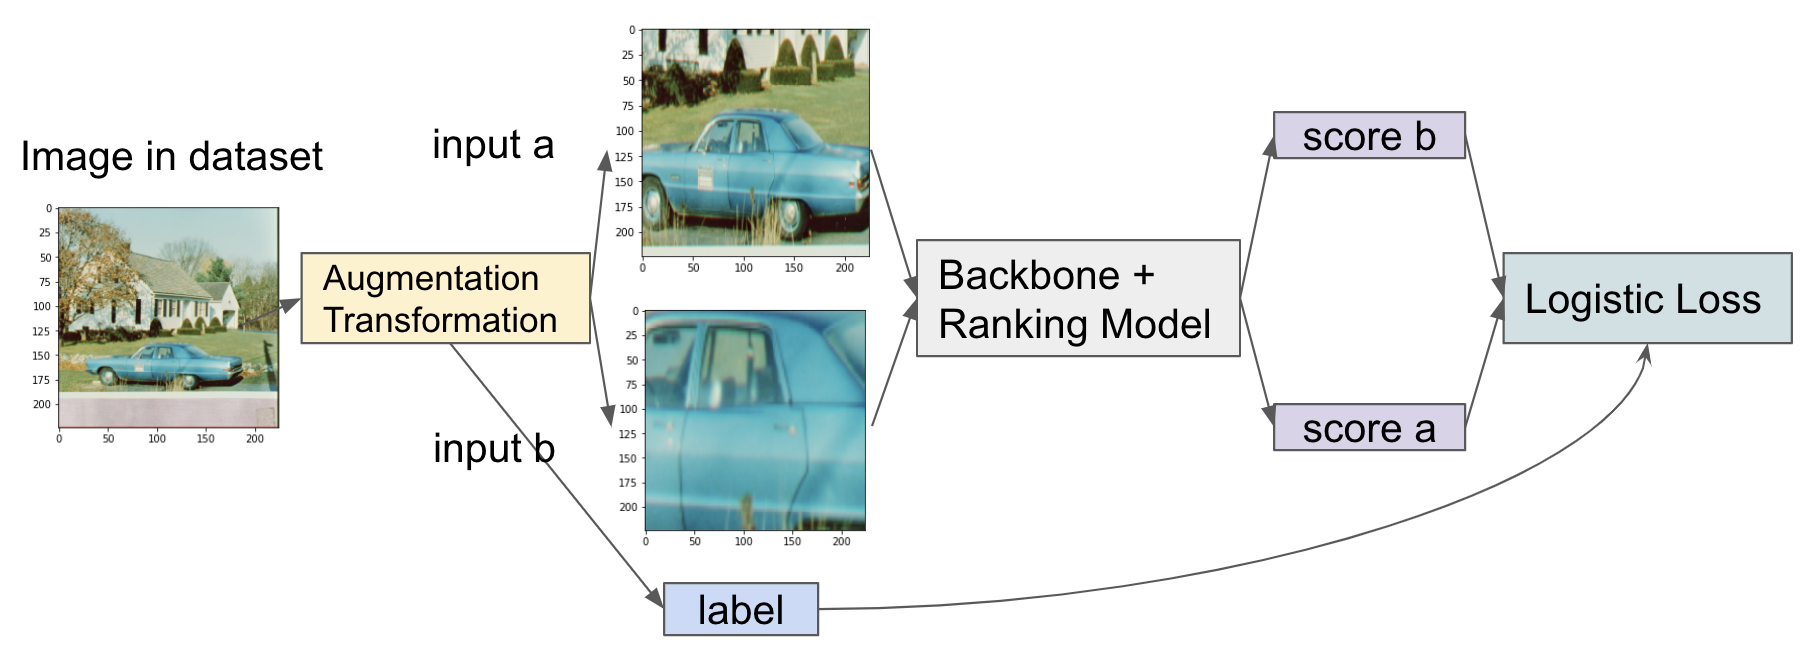
\includegraphics[width=\textwidth]{diagrams/training.png}
\caption{Training pipeline used in our evaluation.}
\label{fig:overview}
\end{subfigure}
\begin{subfigure}[h]{\textwidth}
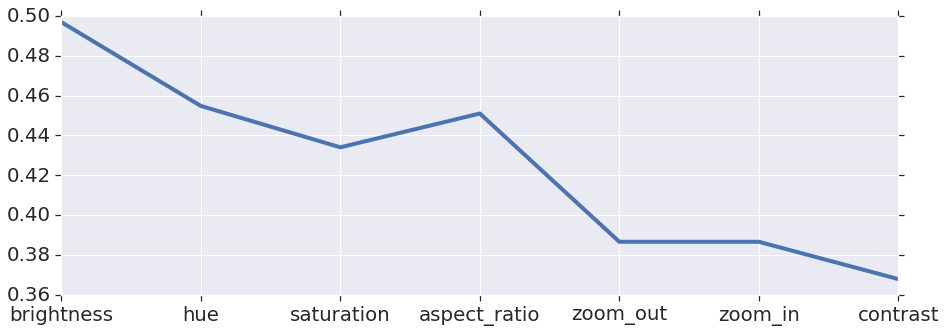
\includegraphics[width=\textwidth]{figures/first_block.png}
\caption{Relative importance of the first block of ResNet-18 for predicting each of the data augmentation ranking tasks.}
\label{fig:importance}
\end{subfigure}
\caption{Can layer activations from CNNs encode input variations introduced by data augmentation? For a given image, a pair of inputs is generated by varying the extent of a data augmentation (e.g., scale), along with a label ranking the extent of the augmentations. The inputs are then fed to a frozen backbone model to extract features for a pairwise ranking model.~\autoref{fig:importance} shows that early ResNet layers are more important for encoding low-level augmentation transformations (brightness and saturation).}
\label{fig:training}
\end{figure}
Convolutional neural networks (CNNs) have enjoyed tremendous success on popular computer vision problems.
Ideally, vision models for these tasks would be equivariant to perturbations such as color, translation, scale, and rotation.
Translation invariance has been partially architected in CNNs~\cite{pmlr-v97-zhang19a}, and building models with other equivariant properties is an active area of research.
These properties include rotation, reflection, and scale among others~\cite{xu2014scale, kanazawa2014locally, cohen2016group, sosnovik2019scale, zhu2019scale, kondor2018generalization}.
In spite of their success, CNN models remain worryingly sensitive to small changes~\cite{goodfellow2014explaining} in the training data with respect to desirable equivariants.
The typical~\cite{krizhevsky2012imagenet}, yet effective ~\cite{zhang2016understanding} approach to build robust models is to leverage brute force via data augmentation.

%Current approaches are ad-hoc, limited
%Tweak this, enahnce understanding
However, current understanding of the effects of data augmentations is limited, and using data augmentations often requires ad-hoc or task-specific heuristics.
%However, applying data augmentation can often require task-specific knowledge to improve model performance.
%For example, a limitation of data augmentation is that augmentation must not shift the training distribution away from the test distribution.
An instance of this problem occurs when objects are shown to models at different scales: popular models for classification exhibit a noticeable drop in accuracy when the scale of their test-time data does not match that of their training-time data~\cite{NIPS2019_9035}.
Here, the proposed heuristic is to finetune the models for the expected distribution of test resolutions---information that may not be easily available.
In parallel, we observe that enhanced data augmentation can lead to dramatic improvements in accuracy, especially in adversarial circumstances~\cite{xie2019adversarial}, but this requires rearchitecting models to effectively leverage adversarial examples.
 

%This phenomenon begs the question of whether reduced performance is the result of limited representation power or limited data.
The importance of data augmentation leads to natural questions about what useful concepts models learn from data augmentations.
%How do model activations respond to input variations presented as data augmentations? What components of model architectures generalize to those variations the most?
As data augmentations are often intended to reflect natural priors (e.g., objects belonging to the same class have variations in scale), a relevant question is how these priors are captured by the model.
Concretely, we ask whether variations corresponding to data augmentations are encoded by models, and where this encoding takes place.
For example, do models encode brightness variations in the earlier layers, in the later layers, or both? 
Which data augmentations correspond to \emph{low-level} model features, and which correspond to \emph{high-level} model features?
%Do they simply become more robust as growing model capacity is leveraged to represent a more varied distribution of inputs, or do models learn to normalize input examples with respect to invariants?
%In the case of scale augmentation: presenting models with objects of different sizes at training time. 
%Are models capable of encoding scale information in their intermediate representations, being starved of sufficient scale diversity during training time, or is their capability for leveraging scale information limited?
%We see answering the question of whether models encode scale information as an important one, because it guides potential research directions aimed at improving the robustness of models.

%If features such as scale and rotation lead to decidedly different activation patterns in models, then a reasonable solution is to design invariance-enhancing architectures to leverage this representation power to route objects of different scales to different parts of the model.
%This possibility suggests that model capacity must be scaled commensurately with the extent of data augmentation.
%On the contrary, if models become better at normalizing input examples with increasing data augmentation, then increased model capacity may not be a strict requirement of increased data augmentation.
%Finally, interpreting what information is captured in intermediate representations of neural networks is useful more generally in understanding neural network behavior and limitations. 


We search for answers to these questions by investigating whether intermediate activations of models capture input differences introduced by data augmentation.
First, we define a set of attributes (scale, aspect ratio, and color transformations) that are desirable invariants (equivariants) for models and commonly targeted by the data augmentation of current computer vision models~\cite{cubuk2019autoaugment}.
%Scale is typically a top priority, with many crops of training set images generated at training time to produce large variation in object scales.
%Rotation is often neglected in data augmentation (other than flipping images).
%Aspect ratio is somewhat implicitly augmented through random cropping of training set images through the distortion that occurs after images are resized.
%Next, we describe a pipeline for evaluating the predictive power of model activations with respect to properties such as scale, rotation, and aspect ratio.
Following these definitions, 
%a definition of the attributes typically transformed by data augmentations, such as scale, aspect ratio, and color,
we propose several experiments, introducing a data augmentation ranking task, as illustrated in Figure~\ref{fig:overview}, to understand whether CNNs implicitly learn a representation for these attributes, comparing against baseline models relying on primitive features.
These experiments measure the predictive performance of a ranking model that uses intermediate features collected from pre-trained models to predict augmentation attributes. Following these experiments, we inspect the relative importance of features used in the ranking model to understand the relative importance of layers in modeling data augmentation attributes.

Our results show that CNNs implicitly learn to encode attributes of popular data augmentations, such as scale, aspect ratio, saturation, and contrast without being explicitly trained on these objectives.
Additionally, we find that these attributes are typically encoded in the earlier layers of networks, suggesting that models learn to normalize input variations introduced by data augmentations. 
Later layers appear relatively more important for aspect ratio and scale, which can be considered higher-level than attributes such as brightness and saturation, as shown in Figure~\ref{fig:importance}.
We present data augmentation prediction as tool to improve the currently limited interpretability~\cite{lipton2018mythos} of CNNs.

%\section{Related Work}
%Data augmentations are a tried and true method of improving CNN performance on fixed-size vision datasets~\cite{ciregan2012multi}~\cite{krizhevsky2012imagenet}.
%Prior work has also compared data augmentation in the input space with augmentations applied in the feature space of neural networks, with the conclusion that ``plausible transformations'' that are guaranteed to avoid changing the label yield the most improvement in model performance~\cite{wong2016understanding}. 
%More recently, using augmentations to incrementally increase the difficulty of training~\cite{2019arXiv191104252X}, automatically generating augmentation strategies~\cite{cubuk2019autoaugment}, and modifying networks to better support adversarial or corruption-based augmentations~\cite{xie2019adversarial} have emerged as promising directions. Other recent lines of work include using augmentation in the semi-supervised setting~\cite{berthelot2019mixmatch}, label-smoothing~\cite{zhang2017mixup}, regularization~\cite{yun2019cutmix, devries2017improved}, and as a means to watermark datasets~\cite{alex2020radioactive}.
%Work has also been done to understand the theoretical motivation behind data augmentation~\cite{dao2019kernel, chen2019grouptheoretic}.
%
%
%On the side of neural network understanding, visualizing features and saliency maps~\cite{erhan2009visualizing, simonyan2013deep, zeiler2014visualizing, Zhou_2016_CVPR, selvaraju2017grad} have enabled interpretation of the functionality and learned patterns of neural network layers.
%Intermediate model features have also been used to synthesize and visualize the textures learned by models by transforming them into position independent Gram matrices and backpropagating on input images to produce the desired feature activations~\cite{lin2016visualizing, gatys2015texture}.
%Automated approaches such as training classifiers to infer brain activity and state are a longstanding staple of neuroscience research~\cite{pereira2009machine}, and have been co-opted recently for understanding fundamental questions about what is encoded in neural network activations~\cite{islam2019much}.
%Apart from augmentation perturbations, evolutionary~\cite{Nguyen_2015_CVPR} and adversarial~\cite{goodfellow2014explaining} perturbations are also automated ways to generate experimental inputs to CNNs.
%
%The tasks of choosing the best model architecture for a task and scaling it appropriately~\cite{pmlr-v97-tan19a} have emerged as important problems, yet both model architecture and model capacity are usually treated as, black-box parameters~\cite{zoph2016neural, real2019regularized}.
%By understanding probing how different components of models react to data augmentation, we hope to reveal which components of models are relevant for good classification performance.
%
\section{A Ranking Model for Augmentations}
To assess whether neural network features encode data augmentation transformations, we propose a ranking task that predicts the \textit{relative} extent of augmentation attributes given intermediate neural network features.
We employ a ranking model instead of a regression approach since obtaining the \textit{absolute} extent of augmentation is difficult.
For example, for the task of predicting the scale of an object, it is difficult to design a numerical definition of scale that is consistent across many different input examples and object classes.
We use a separate ranking model as it facilitates interpretability over blackbox approaches that only consider the final output or accuracy of model predictions.
As we show in~\autoref{sec:importance}, we can leverage the ranking model weights to infer the importance of different layers to the ranking tasks.

\label{sec:ranking_tasks}
To circumvent the requirement of precisely-labeled data for augmentation attributes, we only try to rank the relative values of augmentation attributes.
We use pairwise rank-loss~\cite{chen2009ranking}, which can be considered a binary classification task for pairs of input examples.
For the case of scale, the task is to decide whether the scale of the object in one image is greater than the scale of the object in the other.
More formally, for each $i,j$ pair of examples the loss function is defined as
$$\log{(1 + \exp(-\sgn{(v_i - v_j)} \times (f(x_i)-f(x_j))}))$$
where $v_i, v_j$, $x_i, x_j$, and $f$ denote the true augmentation parameters, input to the ranking model, and ranking model respectively.
This is equivalent to logistic loss where each label is determined by the predicate $v_i > v_j$.
%Each task generates pairs of input images for training and validation by iterating over a subset of the ImageNet dataset.
For each image in the dataset, we produce pairs of images by applying an augmentation transformation parameterized by different random values.

%From this ranking objective, we define seven downstream tasks (scale: (1) zoom in and (2) zoom out, (3) aspect ratio, (4) hue, (5) contrast, (6) saturation, (7) brightness)  focused on data augmentation according to the definitions in ~\autoref{sec:augmentations}.


\section{Choosing and Defining Augmentations}
\label{sec:augmentations}
\begin{figure}
\begin{tabular}[c]{cccc}
    \begin{subfigure}[h]{0.24\textwidth}
    \centering
    \includegraphics[width=\textwidth]{visualizations/img1.png}
    %\caption{}
    \end{subfigure}&
    \begin{subfigure}[h]{0.24\textwidth}
    \centering
    \includegraphics[width=\textwidth]{visualizations/img2.png}
    %\caption{}
    %\label{fig:my_label}
    \end{subfigure}&
    \begin{subfigure}[h]{0.24\textwidth}
    \centering
    \includegraphics[width=\textwidth]{visualizations/img3.png}
    %\caption{}
    \end{subfigure}&
    \begin{subfigure}[h]{0.24\textwidth}
    \centering
    \includegraphics[width=\textwidth]{visualizations/img4.png}
    %\caption{}
    \end{subfigure}\\
    %\begin{subfigure}[b]{0.11\textwidth}
    %\centering
    %\includegraphics[width=\textwidth]{visualizations/img1_rot0.png}
    %\caption{}
    %\end{subfigure}
    %\begin{subfigure}[b]{0.11\textwidth}
    %\centering
    %\includegraphics[width=\textwidth]{visualizations/img1_rot10.png}
    %\caption{}
    %\label{fig:my_label}
    %\end{subfigure}
    %\begin{subfigure}[b]{0.11\textwidth}
    %\centering
    %\includegraphics[width=\textwidth]{visualizations/img1_rot10neg.p%ng}
    %\caption{}
    %\end{subfigure}
    %\begin{subfigure}[b]{0.11\textwidth}
    %\centering
    %\includegraphics[width=\textwidth]{visualizations/img1_rot30.png}
    %\caption{}
    %\end{subfigure}
    \begin{subfigure}[h]{0.24\textwidth}
    \centering
    \includegraphics[width=\textwidth]{visualizations/img1_wider.png}
    %\caption{}
    \end{subfigure}&
    \begin{subfigure}[h]{0.24\textwidth}
    \centering
    \includegraphics[width=\textwidth]{visualizations/img1_wide.png}
    %\caption{}
    %\label{fig:my_label}
    \end{subfigure}&
    \begin{subfigure}[h]{0.24\textwidth}
    \centering
    \includegraphics[width=\textwidth]{visualizations/img1.png}
    %\caption{}
    \end{subfigure}&
    \begin{subfigure}[h]{0.24\textwidth}
    \centering
    \includegraphics[width=\textwidth]{visualizations/img1_tall.png}
    %\caption{}
    \end{subfigure}\\
    %\begin{subfigure}[b]{0.15\textwidth}
    %\centering
    %\includegraphics[width=\textwidth]{visualizations/img2_cut.png}
    %\caption{}
    %\label{fig:my_label}
    %\end{subfigure}
    %\begin{subfigure}[b]{0.15\textwidth}
    %\centering
    %\includegraphics[width=\textwidth]{visualizations/img3_cut.png}
    %\caption{}
    %\label{fig:my_label}
    %\end{subfigure}
    \begin{subfigure}[h]{0.24\textwidth}
    \centering
    \includegraphics[width=\textwidth]{visualizations/img1.png}
    %\caption{}
    \end{subfigure}&
    \begin{subfigure}[h]{0.24\textwidth}
    \centering
    \includegraphics[width=\textwidth]{visualizations/img1_hue0_75.png}
    %\caption{}
    \end{subfigure}&
    \begin{subfigure}[h]{0.24\textwidth}
    \centering
    \includegraphics[width=\textwidth]{visualizations/img1_hue0_5.png}
    %\caption{}
    \end{subfigure}&
    \begin{subfigure}[h]{0.24\textwidth}
    \centering
    \includegraphics[width=\textwidth]{visualizations/img1_hue1_5.png}
    %\caption{}
    \end{subfigure}\\
    \begin{subfigure}[h]{0.24\textwidth}
    \centering
    \includegraphics[width=\textwidth]{visualizations/img1_sat0_5.png}
    %\caption{}
    \end{subfigure}&
    \begin{subfigure}[h]{0.24\textwidth}
    \centering
    \includegraphics[width=\textwidth]{visualizations/img1_sat0_5.png}
    %\caption{}
    \end{subfigure}&
    \begin{subfigure}[h]{0.24\textwidth}
    \centering
    \includegraphics[width=\textwidth]{visualizations/img1.png}
    %\caption{}
    \end{subfigure}&
    \begin{subfigure}[h]{0.24\textwidth}
    \centering
    \includegraphics[width=\textwidth]{visualizations/img1_sat1_5.png}
    %\caption{}
    \end{subfigure}
\end{tabular}
    \caption{Example of our definition of scale (row 1), aspect ratio (row 2), hue (row 3), and saturation (row 4). We order the extent of each augmentation transformation from left to right.
    %$a < b < c < d, e < f = g < h, i < j < k < l$ %Scale increases %from left to right, and is equal top-down. ($c > b > a, a == d, %b == e, c == f$)
    \label{fig:example}}
\end{figure}
We describe our definitions of scale, aspect ratio, hue, contrast, saturation, and brightness in this section, focusing on the constraint that our definitions must yield an ordering or ranking of input examples. ~\autoref{fig:example} shows examples for some augmentations considered.
We choose these augmentations based on the following criteria:
(1) Ease of implementation: given an unlabeled set of images, it is straightforward to infer an ordering of these augmentations For example, smaller crops correspond to a larger view of the same object.
(2) Popularity in training pipelines: each of the transformations considered are either partially or fully implemented in standard TensorFlow~\cite{abadi2016tensorflow}.
(3) Diversity in abstraction level: scale and aspect ratio can be considered higher level image features that require some degree of understanding, whereas color attributes can almost be directly inferred from raw pixel values with limited context.


\subsection{Scale}
\label{sec:scale}
We carefully settle on a narrow definition of object scale, avoiding semantic definitions of scale, especially between different objects.
For example, we are not attempting to assess whether models capture facts such as ``elephants are bigger than dogs.''
We choose a pragmatic definition of scale corresponding to the \emph{solid angle} of an object or the proportion of the field of view occupied by an object.

%We choose this definition so that a model that learns to encode solid angle scale can specialize to examples of different scales. 
This definition of scale captures the problem exhibited by the ``train-test'' resolution discrepancy~\cite{NIPS2019_9035}, where test-time crops of images that occupy a smaller area than training-time crops reduce model accuracy and reflects the random cropping augmentation method that is commonly used to present objects of different scales at training time.
This definition is also distinct from resolution; one can craft arbitrary examples where both high and low resolution images of the same object map to the same scale after they are cropped and resized.

Additionally, we add the qualification that we consider scale to be invariant to occlusion or cropping as long as the object is still partially visible in the frame.
We use this qualification to disentangle scale from the related but separate concept of \emph{bounding-box area} occupied by an object in a frame.
~\autoref{fig:example} gives examples following our definition of scale. 
Section~\ref{sec:augmentations} describes our sampling process and the range of scales considered.
%This qualification is necessary if we rely on this definition of scale to specialize portions of models for different scales.
%TODO: add a figure showing exmaples where scale a $>$ scale b, scale a == scale b, etc.
%\subsection{Rotation}
%The rotation augmentation rotates images either clockwise or counterclockwise from their original position.
%To disentangle rotation from other augmentations such as vertical/horizontal flips, we only apply rotation at angles less than 45 degrees and use the absolute value of rotation angle for ranking.
%As flipping an image is a common augmentation for many off-the-shelf models trained on ImageNet, we avoid differentiating between counterclockwise and clockwise rotation.
%Instead, we simply consider rotation to be ordered based on the offset from the vertical axis. with a maximum value of $\frac{pi}{4}$ radians.
%The intrinsic variation of object orientation in the dataset is likely to make rotation a noisy augmentation to probe accurately---we use our definition under the assumption that the distribution of object orientations in ImageNet is not uniform.
%More intuitively, our definition asks the model to rank the likelihood of two orientations given two images of the same object.

%\paragraph{Scale Ranking Tasks}
From this definition of scale, we define two ranking tasks: ``zoom-out'' and ``zoom-in.''
For the ``zoom-out'' task, we generate pairs of input images that zoom-out from the bounding boxes of objects to generate input images with different scales.
We uniformly sample two values in the range $[0.1, s]$, where $s$ is the smallest of the total vertical or horizontal distance from the border of the bounding box to the boundaries of the image.
For the images in the dataset we use (\autoref{sec:dataset}), $s$ is expected to be at least $0.3$.
For the ``zoom-in'' task, the different scales are generated by zooming-in on bounding boxes to different extents.
We uniformly randomly sample two values in $[0.5, 0.9]$ that determine the fraction of the bounding box to trim before resizing the result to the input size of the backbone model $224\times224$ for each pair of inputs.
We define the zoom-in and zoom-out tasks separately because although they may be of similar difficulty for a human evaluator, intuitively the zoom-out task may be easier as the area occupied by an object is a highly accurate proxy for scale when the object of interest does not occupy the entire frame.


\subsection{Aspect Ratio}
Models are naturally exposed to a range of aspect ratios of objects at training time through random cropping and natural variation in the input distribution.
Random cropping is an important source of aspect ratio variation, as many augmentation pipelines do not consider the original aspect ratios of objects as a constraint on the crop dimensions.
With respect to aspect ratio, we define the ranking order from wide to thin, or the ratio of vertical to horizontal pixels present in the input after cropping (but before resizing).
Note that while ordering the aspect ratio between two arbitrary objects is difficult, and this definition suffices when only considering different crops of the same object.
%As with the rotation case, we postulate that the presence or absence (e.g., of extreme aspect ratios) in the training distribution will be a factor in how the model reacts to aspect ratio augmentation.

%\paragraph{Aspect Ratio Ranking Task}
The aspect ratio task uses the same pipeline as the scale tasks, with the objective changed to ranking the ratio of vertical to horizontal pixels.
To generate each input image, we sample four random uniform values in $[0.4, 0.4]$ that determine the number of horizontal and vertical pixels to trim from each input image.

\subsection{Hue, Saturation, Contrast, Brightness}
\label{sec:define_color}
Hue, saturation, and contrast are common distortions applied to input images.
As each of these augmentations are parameterized by either relative multipliers or absolute deltas to the original image, these parameters lend themselves naturally to an ordering for ranking.
%Section~\ref{sec:augmentations} details the range of hue, saturation, contrast, and brightness values we sample. 
We include brightness as a sanity check that should be trivially encoded for both the CNN backbones and baselines.
While we consider contrast a color transformation, it is arguably higher-level than the other augmentations as discerning contrast requires non-local information.
%\paragraph{Hue, Saturation, Contrast, Brightness Ranking Tasks}

We again sample of random uniform values for each ranking task.
For both saturation and contrast, we sample the relative multipliers used to apply the transformation to determine the ranking labels (in the range $[0.5, 1.5]$).
For hue, we rank the delta relative to the original image (in the range $[-0.2, 0.2]$).


%\subsection{MixUp}
%Another axis of augmentation that has been recently explored (e.g., in MixUp~\cite{zhang2017mixup} and CutMix~\cite{yun2019cutmix}) involves mixing classes of objects for label smoothing.
%As we use pretrained models with frozen parameters, it is difficult to apply label smoothing approaches directly (i.e., by mixing labels) without sacrificing comparability against the other augmentations.
%However, we can leverage the knowledge that some object categories, such as human faces are not in the ILSVRC 2012 label set yet known to be cues for certain object categories.
%From this knowledge, we propose a mixing objective that blends the input image with an image of a human face with ratios $\lambda$ and $(1-\lambda)$ respectively.
%This augmentation provides an easy ranking (using the value of $\lambda$) without altering the ground-truth labels of the dataset.
%We include this augmentation as it is expected to be one that is likely to require abstract or high level features.

\begin{figure}
    \begin{subfigure}[b]{0.32\textwidth}
    \centering
    \includegraphics[width=\textwidth]{visualizations/img1_dct.png}
    \caption{}
    \label{fig:my_label}
    \end{subfigure}
    \begin{subfigure}[b]{0.32\textwidth}
    \centering
    \includegraphics[width=\textwidth]{visualizations/img2_dct.png}
    \caption{}
    \label{fig:my_label}
    \end{subfigure}
    \begin{subfigure}[b]{0.32\textwidth}
    \centering
    \includegraphics[width=\textwidth]{visualizations/img3_dct.png}
    \caption{}
    \end{subfigure}
    \caption{Average magnitude of frequency coefficients of an $8 \times 8$ DCT applied patch-wise to images at increasing scales (from left to right). Frequency coefficients are ordered in a zig-zag pattern, with lowest frequency in the top left and highest frequency in the bottom right. The magnitude of higher frequency coefficients decreases as scale increases.}
    \label{fig:dct}
\end{figure}



\section{Methodology}
To understand whether CNN activations capture attributes of data augmentations, we adopt an experiment pipeline similar to one used to extract position information from CNNs~\cite{islam2019much}.
We also use the intermediate activations as input to a predictor from a pre-trained vision model with frozen parameters, but with several key differences.
Instead of attempting to generate a two-dimensional output, our prediction task is learning to rank input examples according to their data augmentations.
Our ranking model uses only average pooling and a single linear layer to allow easy interpretation of the model weights.
In the case of position information, the ground-truth can be generated deterministically, and it is the same across all images.
However, in the case of general data augmentation, ranking labels are generated on-the-fly, in tandem with the augmentations.





%The rotation task uses this same data generation pipeline, with the objective changed to ranking the relative rotation of input images.


%We choose images that contain only a single bounding box to avoid producing crops that contain multiple instances of the same object at different scales, and only choose bounding boxes that give enough slack to both ``zoom-in'' from the bounding box and ``zoom-out'' of the bounding box without overstepping the boundaries of the image.


\subsection{Dataset}
\label{sec:dataset}
We use a subset of the ImageNet~\cite{deng2009imagenet} training dataset in our experiments.
Specifically, we limit our subset to images that have exactly one bounding box to mitigate the effect of partially cropping only some objects in view.
We also choose images with bounding boxes that span at least $30\%$ of the input image, with the additional requirement that the borders of the bounding box must be at least $30\%$ of the image dimensions away from edges of the image.
Together, these requirements ensure that there is range to zoom out from bounding boxes and to provide reasonable resolution when zooming in on a bounding box.
These constraints reduce the original $1.2$ million image ImageNet dataset to roughly $86,000$ images, which we split into a $65,000$ image training set and a $21,000$ image validation set.
For simplicity, we use this dataset for all of our ranking tasks, even those that do not require bounding box constraints.

\subsection{Baseline Comparisons}
We also evaluate two baselines that either use an $8\times8$ discrete cosine transform (DCT) to generate features (to understand the impact of frequency information), or are passed the input images directly (passthrough).
~\autoref{fig:dct} shows an example of how the magnitude of frequency coefficients change with the scale of an object.
For the DCT baseline, we apply average pooling to the DCT features while the spatial dimensions of the passthrough baseline are not reduced.



\subsection{Ranking Model and Training Pipeline}
\begin{figure}[t]
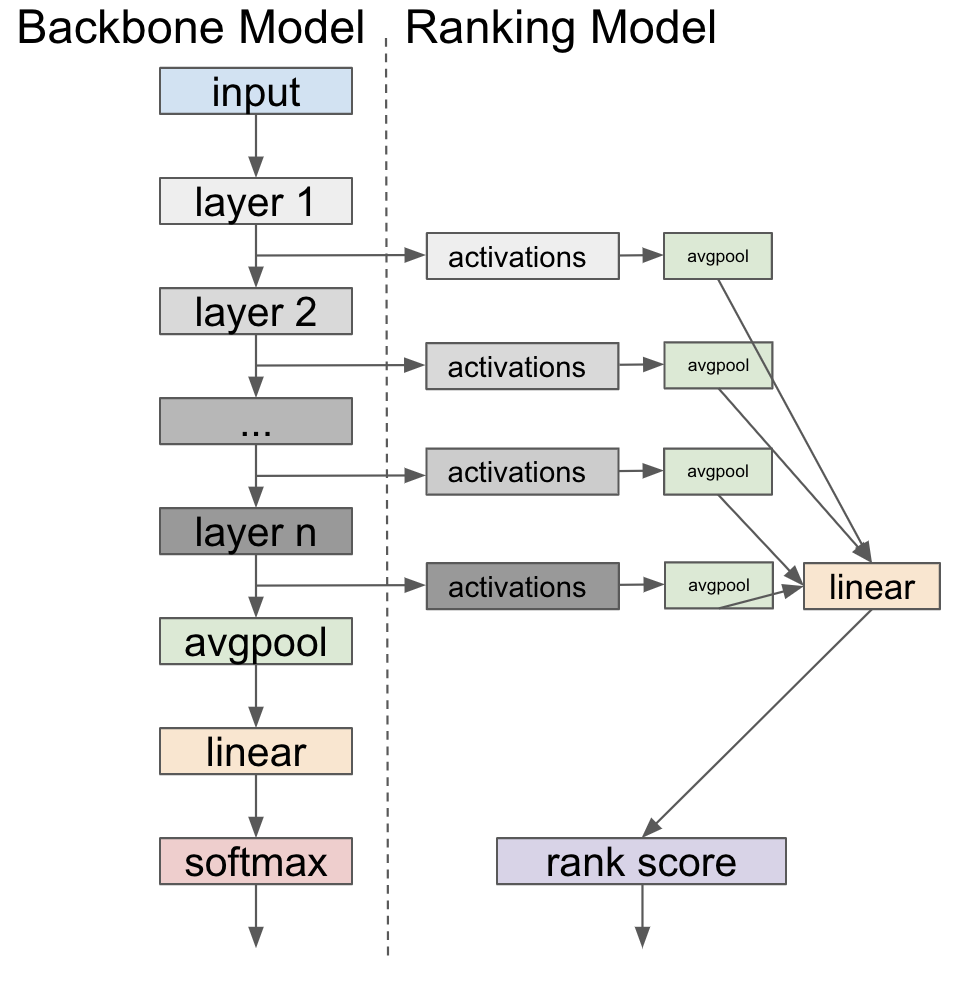
\includegraphics[width=\textwidth]{diagrams/ranking.png}
\caption{Backbone and ranking model used in our evaluation. The backbone model is a pre-trained CNN (such as ResNet-18), with parameters frozen. The activations from the backbone are average-pooled to align their spatial dimensions and fed to a linear layer that produces a score for the ranking objective.}
\label{fig:ranking}
\end{figure}

Our ranking model uses the intermediate activations from a pre-trained CNN as inputs to rank instances of a given data augmentation transformation.
~\autoref{fig:ranking} shows a high-level diagram of the relationship between the backbone model and the ranking model.
For our experiments, we use ResNet-18/50~\cite{he2016deep} as the backbone, although this approach is compatible with any feedforward CNN.
To unify the spatial dimensions of each layer, we apply global average pooling to reduce each activation tensor to a tensor with $1\times 1$ spatial resolution, preserving the channels.
The average-pooled tensors are then fed to a single linear layer that computes the ranking score for a given input example.
For each each pair of input examples, we use the ranking scores and logistic loss to fit the linear layer's parameters.



The training pipeline begins with iteration through a dataset of images, where each image is used to generate a pair of input examples.
Each input example is transformed according by sampling a random variable and the current augmentation ranking task (e.g., scale).
At this time, a label for this pair of input examples can be computed as a boolean expression of the random variables (e.g., scale\_a $>$ scale\_b?).
A collection of pairs and labels comprise a batch that is used to fit the linear layer with logistic loss.
Note that the parameters of the backbone model are frozen during training of the ranking model to prevent the ranking task from affecting the intermediate features of the backbone.
We use the same approach with the baselines, with average pooling omitted for the passthrough baseline.

\subsection{Where are data augmentations encoded?}
We use the weights of the linear layer to measure the relative importance of the activations for each layer of the backbone model.
Due to the simplicity of the linear ranking model, we can measure the contribution of each layer of the backbone by taking the product of the weights and the corresponding standard deviation in the layer activations.

\section{Evaluation}
We begin the evaluation with the accuracy results (\autoref{tab:accs}) for each of the pairwise ranking tasks.
Due to the binary nature of a pairwise ranking task, the accuracy of random guessing is $50\%$.
For all tasks, we find that the ResNet backbones either match or substantially outperform the baselines, particularly on the augmentations that do not manipulate color.  This suggests CNNs may implicitly model scale and aspect ratio as components of features.

Prior work has compared the early layers of CNN to the discrete cosine transform (DCT) ~\cite{gueguen2018faster}.
To some extent, we expect the DCT~(\autoref{fig:dct}) and low-level features of earlier layers to act as a proxy for scale and/or aspect ratio.
Intuitively, two views of the same object at different scales are expected to contain different frequency domain representations, where the smaller scale view is expected to have more high frequency components than the larger scale view.
The details of the object exhibit higher spatial frequency as they appear finer in the image. 
If CNNs capture some elements of frequency domain transforms in convolution layers, we would expect that this information could be used to better infer scale information.
%Similarly, aspect ratio can potentially be modeled using a combination of horizontal and vertical spatial frequency features.
%Bounding box information (predicted by detection backbones) is correlated with aspect ratio, and extremes of aspect ratios are unlikely to be in the input distribution seen by the model at training time.
Other augmentations, such as hue and saturation, may present cues in the absolute or relative values of the color channels early in network architectures.


\begin{table}[t]
\begin{center}
\begin{tabularx}{\textwidth}{  | >{\raggedright\arraybackslash}X 
  | >{\centering\arraybackslash}X 
  | >{\raggedleft\arraybackslash}X |} 
 \hline
  & Zoom In-Train & Zoom In-Val \\ 
 \hline
 Passthrough & 97.7 & 46.4 \\ 
 \hline
 DCT & 56.8 & 46.6 \\ 
 \hline
 ResNet-18 & 93.9 & \textbf{90.1} \\ 
 \hline
 ResNet-50 & 90.8 & 84.9 \\ 
 \hline
\end{tabularx}
\begin{tabularx}{\textwidth}{  | >{\raggedright\arraybackslash}X 
  | >{\centering\arraybackslash}X 
  | >{\raggedleft\arraybackslash}X |} 
 \hline
  & Zoom Out-Train & Zoom Out-Val\\ 
 \hline
 Passthrough & 98.5 & 51.8 \\ 
 \hline
 DCT & 57.5 & 52.4 \\ 
 \hline
 ResNet-18 & 82.4 & \textbf{68.8} \\ 
 \hline
 ResNet-50 & 77.6 & 64.8 \\ 
 \hline
\end{tabularx}
\begin{tabularx}{\textwidth}{  | >{\raggedright\arraybackslash}X 
  | >{\centering\arraybackslash}X 
  | >{\raggedleft\arraybackslash}X |} 
 \hline
  & Aspect Ratio-Train & Aspect Ratio-Val\\ 
 \hline
 Passthrough & 98.7 & 54.9 \\ 
 \hline
 DCT & 54.1 & 57.7 \\ 
 \hline
 ResNet-18 & 87.6 & 80.9 \\ 
 \hline
 ResNet-50 & 85.9 & \textbf{81.3} \\ 
 \hline
\end{tabularx}
\begin{tabularx}{\textwidth}{  | >{\raggedright\arraybackslash}X 
  | >{\centering\arraybackslash}X 
  | >{\raggedleft\arraybackslash}X |} 
 \hline
  & Hue-Train & Hue-Val\\ 
 \hline
 Passthrough & 94.0 & 65.0 \\ 
 \hline
 %DCT & 65.1 & 69.9 \\ 
 %\hline
 ResNet-18 & 87.6 & \textbf{71.6} \\ 
 \hline
 ResNet-50 & 84.0 & 66.0 \\ 
 \hline
\end{tabularx}
\begin{tabularx}{\textwidth}{  | >{\raggedright\arraybackslash}X 
  | >{\centering\arraybackslash}X 
  | >{\raggedleft\arraybackslash}X |} 
 \hline
  & Saturation-Train & Saturation-Val\\ 
 \hline
 Passthrough & 97.5 & 98.9 \\ 
 \hline
 %DCT & 97.5  & 98.9 \\ 
 %\hline
 ResNet-18 & 97.5 & 98.3 \\ 
 \hline
 ResNet-50 & 95.2 & 94.0 \\ 
 \hline
\end{tabularx}
\begin{tabularx}{\textwidth}{  | >{\raggedright\arraybackslash}X 
  | >{\centering\arraybackslash}X 
  | >{\raggedleft\arraybackslash}X |} 
 \hline
  & Contrast-Train & Contrast-Val\\ 
 \hline
 Passthrough & 100.0 & 62.0 \\ 
 \hline
 %DCT & 59.2 & 40.2 \\ 
 %\hline
 ResNet-18 & 100.0 & \textbf{100.0}\\ 
 \hline
 ResNet-50 & 99.7 & 99.7\\ 
 \hline
\end{tabularx}
\begin{tabularx}{\textwidth}{  | >{\raggedright\arraybackslash}X 
  | >{\centering\arraybackslash}X 
  | >{\raggedleft\arraybackslash}X |} 
 \hline
  & Brightness-Train & Brightness-Val\\ 
 \hline
 Passthrough & 100.0 & 100.0 \\ 
 \hline
 %DCT & 100.0 & 100.0 \\ 
 %\hline
 ResNet-18 & 100.0 & 100.0 \\ 
 \hline
 ResNet-50 & 99.3 & 98.8 \\ 
 \hline
\end{tabularx}
\end{center}
\caption{Accuracies for ranking models that use the baselines and ResNet backbones across the ranking tasks. ResNet features encode many augmentation attributes to a high degree of accuracy, particularly high-level ones such as scale and aspect ratio. ResNet features also beat the baselines on contrast by a wide margin. The accuracy of the ranking model can be used as a proxy to determine to what degree an augmentation attribute is encoded in the CNNs.}
\label{tab:accs}

\end{table}
When comparing results for the scale tasks, we note that the performance of the ResNet backbone was substantially lower for the ``zoom-out'' than ``zoom-in'' task.
This drop in accuracy was surprising as it was thought that the ranking model could rely on the later layers and localization as a proxy for scale, although it is possible that the use of average pooling in the ranking model could have limited localization information.
Additionally, performance on the zoom-out task may have suffered as a consequence of it being more fine-grained than the zoom-in task: many images may have a limited amount of slack in which crop sizes can be increased without overstepping image boundaries.
Still, the performance of the ResNet backbones far surpassed the DCT baseline on both scale tasks, suggesting that CNNs have stronger cues for object scale than spatial frequency.

This result suggests another source of scale information may appear in the higher-level representations of networks.
With the knowledge that activations late in CNNs (e.g., at the last layer) map neatly to class labels~\cite{Zhou_2016_CVPR}, it is plausible that high-level features map coarsely to scale as well (e.g., objects that are large on average or small on average).
%We can systematically probe the existence of scale information by sequentially including activations from deeper layers in feedforward models.
However, we attempt to avoid trivial cues for scale via a very simple ranking model (\autoref{fig:ranking}) and by applying average pooling to the activations before ranking.
%Rotation can likely be partially inferred from existing CNN features if we consider that typical off-the-shelf models do not see significant data augmentations with respect to rotation in their input training distribution.
%From this assumption, we expect high level model features (such as the last layer) to vary with rotation as plausible orientations of objects (low rotation angle) cause the model to output higher probability values than more extreme orientations of objects (high rotation angle).

%Similarly, aspect ratio can potentially be be modeled using a combination of horizontal and vertical spatial frequency features.
%Bounding box information (predicted by detection backbones) is correlated with aspect ratio, and extremes of aspect ratios are unlikely to be in the input distribution seen by the model at training time.

%Other augmentations, such as hue and saturation, may present cues in the absolute or relative values of the color channels early in network architectures.

Across some tasks, we observe that the ranking using the ResNet-18 backbone sometimes outperforms the ResNet-50 backbone.
We suspect that this is due to the large increase in the number of input dimensions to the ranking model when ResNet-50 is used (due to the increase in total number of channels), and regularizing the weights of the ranking model could yield improved performance.
The heavy overfitting of the passthrough baseline can likely be attributed to reliance on absolute position (no average pooling is used) that is not generalizable to the validation set.
An alternative hypothesis is that ResNet-50 yields lower ranking performance because it more successfully normalizes away perturbations caused by augmentations.
This hypothesis is interesting as it suggests that models with stronger performance may do a better job of eliminating differences created by data augmentations.

Hue appears to be the least favorable task for the ResNet backbones (relative to the baselines).
We suspect that this may be due to the narrow range of hue considered, or the difficultly in assessing the absolute delta in hue from the original image.
We expect the easier task of ranking the raw value of hue rather than the magnitude to be easier.
On the opposite end, contrast appears to be the least favorable task for the baselines (relative to the ResNet backbones), especially of the color augmentations.
We expect that this is because contrast describes the image as a whole and consequentially is a higher-level attribute than hue or saturation.
Accordingly, contrast depends more on later layers of the backbones than the other color transformations~(\autoref{fig:resnet18and50}).


We find that the baseline backbones achieve their highest performance on the color tasks.
This is relatively unsurprising, as some color attributes (such as saturation) may be discernible by the raw values of the input color channels.
More surprisingly, however, was that while the early layers were favored especially for the color-focused transformations, the most highly weighted layer was not the stem of the ResNet, models but rather a few layers later.


\subsection{Which layers encode the augmentations?}
\label{sec:importance}
\begin{figure*}
\begin{center}
\begin{subfigure}[h]{0.49\textwidth}
    \centering
    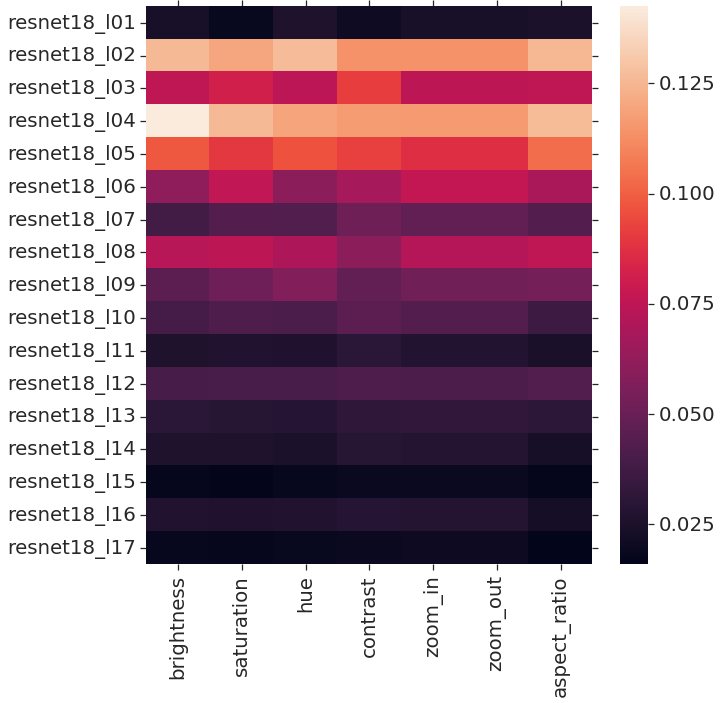
\includegraphics[width=\textwidth]{figures/resnet18_mean_new.png}
    \caption{}
    \label{fig:resnet18_mean}
\end{subfigure}
%\hspace{0.5in}
\begin{subfigure}[h]{0.49\textwidth}
    \centering
    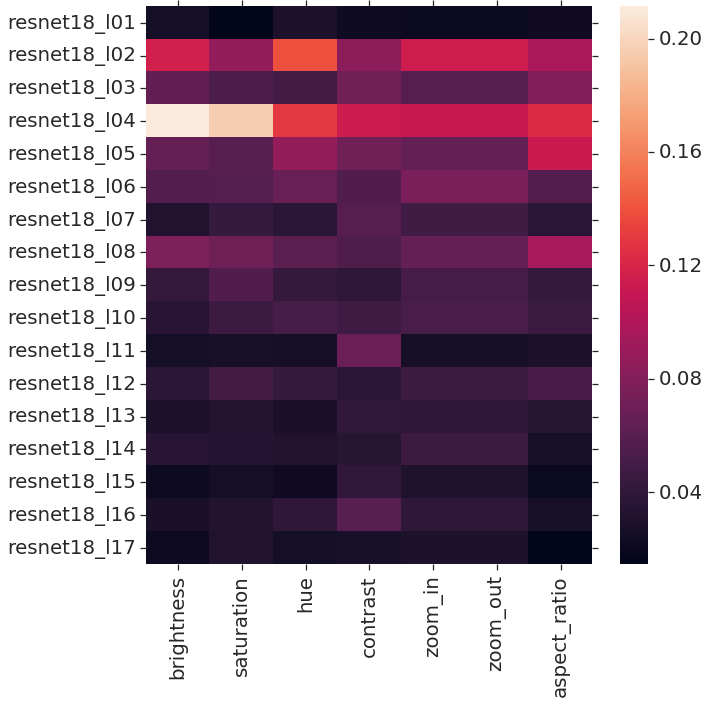
\includegraphics[width=\textwidth]{figures/resnet18_max_new.png}
    \caption{}
    \label{fig:resnet18_max}
\end{subfigure}
\begin{subfigure}[h]{0.49\textwidth}
    \centering
    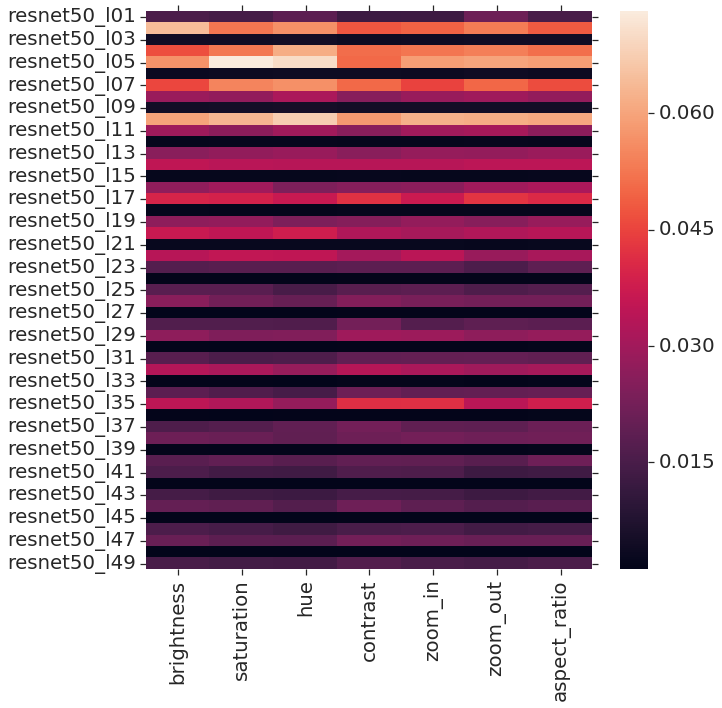
\includegraphics[width=\textwidth]{figures/resnet50_mean_new.png}
    \caption{}
    \label{fig:resnet50_mean}
\end{subfigure}
%\hspace{0.5in}
\begin{subfigure}[h]{0.49\textwidth}
    \centering
    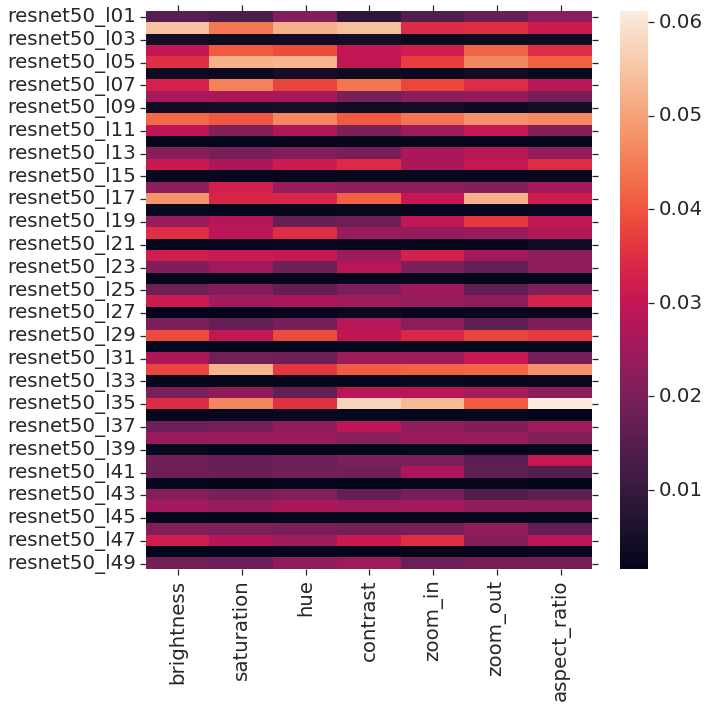
\includegraphics[width=\textwidth]{figures/resnet50_max_new.png}
    \caption{}
    \label{fig:resnet50_max}
\end{subfigure}
\end{center}
\caption{Weightings of activations for ranking tasks with a ResNet-18 backbone (a, b) and ResNet-50 backbone (c, d), with the sum of each task normalized to 1.0. Ranking tasks are ordered from left to right roughly from low-level (color perturbations) to high-level (scale and aspect ratio). Early layers are more important for lower-level ranking tasks, such as color attributes. Color  represents mean (a, c) and max (b, d) value across channels.}
\label{fig:resnet18and50}
\end{figure*}
\autoref{fig:resnet18_mean} and~\autoref{fig:resnet18_max} show the relative importance of ResNet-18 layers for the ranking tasks when taking the mean and max across the channels respectively.
A general trend is that the earlier layers are weighted more highly for all of the ranking tasks.
Interestingly, this trend occurs even when taking the max across channels despite the later layers having more channels than the early layers.

Another difference is that slightly deeper layers appear more important (or alternatively, early layers are less important) for contrast, aspect ratio and scale (zoom in and zoom out).
This pattern may be the result of contrast, scale, and aspect ratio being a higher-level attribute than brightness and saturation.
%\begin{figure*}[t]
%\caption{Weightings of activations for ranking tasks with a ResNet-50 backbone. Again, we find that early layers are more important for ranking lower-level attributes. Later layers appear to be more highly utilized than in ResNet-18. Color represents mean (a) and max (b) value across channels.}
%\label{fig:resnet50}
%\end{figure*}
We see a similar trend for the mean (\autoref{fig:resnet50_mean}) and max (\autoref{fig:resnet50_max}) of feature importance across channels for ResNet-50.
For the aspect ratio and zoom in tasks, the most highly weighted layer (when taking the max across channels) occurs later in the model.
In both ResNet-18 and ResNet-50, shortcut layers seem to be neglected by the ranking models.
In ResNet-50, however, the later layers appear to be more highly utilized (especially when taking the maximum across channels) than in ResNet-18 though this effect might be accounted for by ResNet-50's greater number of channels increasing the chances that some channel in a layer may be weighted highly.

To further validate the trend of early layers more strongly encoding augmentation attributes, we rerun a selection of experiments, using activations from only a few ResNet-18 layers at a time.
If the early layers are more relevant for capturing or encoding augmentation attributes, then we should observe a drop in accuracy when using activations from later layers.
Indeed,~\autoref{tab:halfs} shows this drop, suggesting that even if neural networks encode augmentations, this signal begins to be normalized away in later layers, a trend we discuss further in~\autoref{sec:specialization}.
%That suggesting that regularization may further improve the performance of the ResNet backbones.


\begin{table}[tb]
\begin{center}
\begin{tabularx}{\textwidth}{  | >{\raggedright\arraybackslash}X 
  | >{\centering\arraybackslash}X 
  | >{\raggedleft\arraybackslash}X |} 
 \hline
 & Zoom In-Train & Zoom In-Val\\ 
 %\hline
 %ResNet-18 1st$\frac{1}{2}$& 95.3 & \textbf{91.0} \\ 
 %\hline
 %ResNet-18 2nd$\frac{1}{2}$& 91.7 & 86.9 \\
 % \hline
 %ResNet-18 Both & 93.9 & 90.1 \\  
 %\hline
 ResNet-18 Block 1& 95.5 & 92.2\\
 \hline
 ResNet-18 Block 2& 95.8 & \textbf{92.8}\\
 \hline
 ResNet-18 Block 3& 93.7 & 89.1\\
 \hline
 ResNet-18 Block 4& 93.2 & 90.0\\
 \hline
 ResNet-18 Block 5& 90.0 & 85.1\\
 \hline
 ResNet-18 Block 6& 87.5 & 82.9\\
 \hline
\end{tabularx}
\begin{tabularx}{\textwidth}{  | >{\raggedright\arraybackslash}X 
  | >{\centering\arraybackslash}X 
  | >{\raggedleft\arraybackslash}X |} 
 \hline
 & Aspect Ratio-Train & Aspect Ratio-Val\\ 
 %\hline
 %ResNet-18 1st$\frac{1}{2}$& 92.6 & \textbf{91.8} \\ 
 %\hline
 %ResNet-18 2nd$\frac{1}{2}$ & 83.7 & 74.2 \\
 % \hline
 %ResNet-18 Both & 87.6 & 80.9 \\
 %\hline
 ResNet-18 Block 1& 75.7 & 78.7 \\
 \hline
 ResNet-18 Block 2& 87.6 & 86.3 \\
 \hline
 ResNet-18 Block 3& 86.5 & \textbf{88.8}\\
 \hline
 ResNet-18 Block 4& 87.7 & 87.2 \\
 \hline
 ResNet-18 Block 5& 80.1 & 79.1 \\
 \hline
 ResNet-18 Block 6& 66.7 & 62.8 \\
 \hline
\end{tabularx}
\begin{tabularx}{\textwidth}{  | >{\raggedright\arraybackslash}X 
  | >{\centering\arraybackslash}X 
  | >{\raggedleft\arraybackslash}X |} 
 \hline
 & Hue-Train & Hue-Val\\ 
 \hline
 %ResNet-18 1st$\frac{1}{2}$& 78.9 & \textbf{72.9} \\ 
 %\hline
 %ResNet-18 2nd$\frac{1}{2}$& 86.9 & 68.4 \\
 %\hline
 %ResNet-18 Both & 87.6 & 71.6 \\
 %\hline
 ResNet-18 Block 1& 75.1 & \textbf{77.5} \\
 \hline
 ResNet-18 Block 2& 77.6 & 76.6 \\
 \hline
 ResNet-18 Block 3& 77.8 & 73.0 \\
 \hline
 ResNet-18 Block 4& 81.0 & 72.5 \\
 \hline
 ResNet-18 Block 5& 82.5 & 67.5 \\
 \hline
 ResNet-18 Block 6& 82.1 & 65.8 \\
 \hline
\end{tabularx}
\caption{Ranking accuracy when only using features from a block of ResNet-18, ordered from early to later layers. The early blocks yield higher accuracy, indicative of early layers more strongly encoding augmentation attributes.}
\label{tab:halfs}
\end{center}
\end{table}




\section{Discussion}

\paragraph{Specialization vs. normalization}
\label{sec:specialization}
For augmentations that are encoded or captured by CNN activations, we ask \emph{where} or at what depth?
We describe this question as the specialization vs. normalization question: we posit that data augmentations that are encoded by earlier layers are \emph{normalized} away by the model, whereas attributes that are encoded in later layers incur \emph{specialization}.
Intuitively, if a model captures augmentation attributes in early layers but discards this information by the later layers, it has normalized away the augmentation.
However, if a model retains augmentation differences in later layers, the intuition is that this augmentation incurs specialization in the same way that the last layer is specialized at a per-class granularity.

%The distinction between specialization and normalization has been partially observed in applications of mixtures-of-experts models such as  CondConv~\cite{NIPS2019_8412}, where each layer in a feedforward is replaced with a dynamic combination of ``experts.''
%In the case of CondConv, it was observed that the distribution of the experts weights varied more in the later layers of the model, indicating greater specialization among the experts in later layers.

The importance of activations from earlier layers relative to those from later layers for our ranking objectives suggests that attributes such as scale are normalized away by CNNs.
This phenomenon appears more desirable than the alternative where augmentation attributes are encoded and preserved throughout the model, indicating limited generalization at the output.
The lower ranking accuracy when using a ResNet-50 backbone (vs. ResNet-18) may indicate that more accurate models do a better job of normalizing away augmentations.
%That models capture scale information should be a reassurance that they do not simply perform classification by memorizing textures at different scales.

\paragraph{An adversarial ``ranking model''}
An alternative we considered was a GAN that proposes augmented images that attempt to fool the backbone model, taking activations of a pre-trained backbone as input.
However, a difficulty of this approach is that some popular augmentations (scale transformations) are not easily expressible using standard vision operators or are not differentiable.
Still, we see adversarial augmentations as an important related problem: what augmentations are the most difficult for current models?
%TODO: compare the GAN. Augmentations are not always differentiable. Justification for the choice of ranking models. Generator of GAN would generated augmented images. And the pre-trained network will be used to classify normal vs augmented ones. 

\paragraph{Can ranking objectives be used as pre-training tasks?}
\begin{figure}
    \centering
    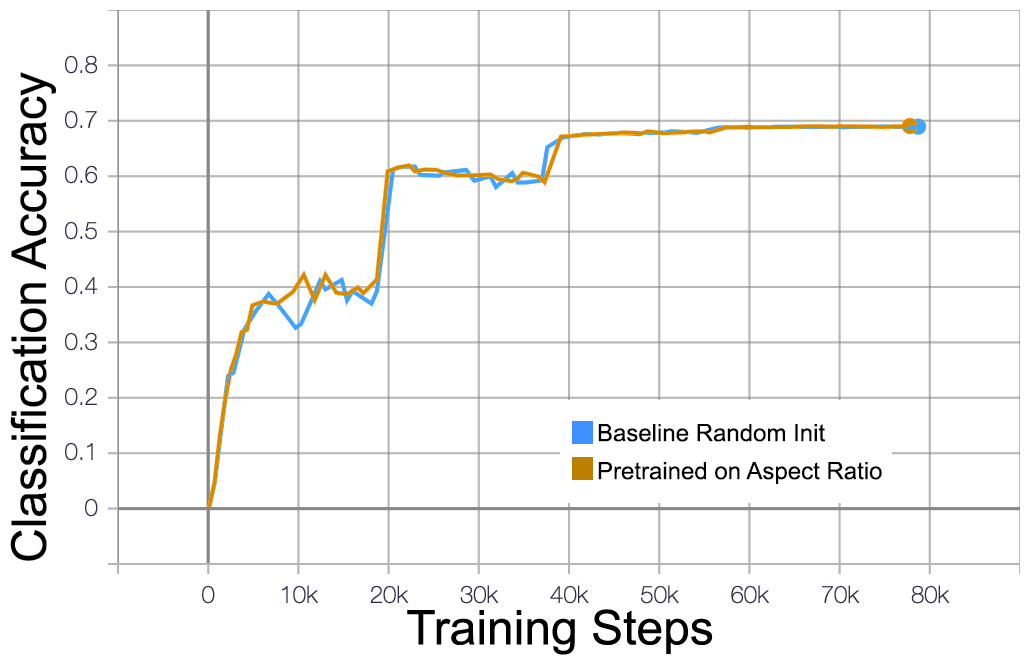
\includegraphics[width=\textwidth]{figures/dev_accuracy_labels.png}
    \caption{ImageNet classification accuracy vs. training steps of a from-scatch model compared to that of a backbone model pre-trained on the aspect ratio ranking task. Classification performance does not improve, suggesting that encoding augmentations is not inherently desirable.}
    \label{fig:pretraining}
\end{figure}
%From a human vision perspective, it would be unsurprising that neural networks implicitly learn to encode common data augmentation transformations such as scale and aspect ratio, as these are almost instinctive qualities of human vision.
That neural networks appear to encode data augmentation transformation attributes raises the question of whether these attributes are inherently useful for vision tasks.  
If it is useful for neural network models to encode these attributes, would a source of accurate scale, aspect ratio, or color information improve their performance?
%The concept of useful auxiliary tasks has similarities to pre-training objectives in natural language processing, where models can leverage massive corpuses of text in a semi-supervised fashion. Like pre-training objectives for language models, the ranking objectives presented in this paper require little annotation or labeled data.
%We ignore the class labels of the ImageNet dataset and only use bounding box reduction as a means of reducing noise in our experiments.
~\autoref{fig:pretraining} shows the results of an experiment where a backbone is pre-trained without class labels via the downstream ranking task (aspect ratio).
We find that pre-training to rank augmentations does not improve classification performance, with no improvement over training from scratch.
The lack of improvement seems to support the hypothesis that the ability to encode augmentations is not inherently desirable, and that normalization is the desired effect.
%A potential application of these properties would be to apply the data augmentation ranking objectives to unlabeled images, then finetuning them for downstream computer vision tasks.


%\paragraph{Can we design better neural network architectures?}
%An interesting question is whether performance on ranking tasks is a proxy for sufficient model capacity %in early model layers.
%If we can use objectives such as the ability to encode transformations such as scale and color, is this a %useful metric for sizing earlier network layers?



\paragraph{Limitations and future work}
In using a simple linear layer to build our ranking model, we sacrifice model performance for interpretability.
It may be entirely possible that with sufficient representation power in the ranking model, data augmentation transformations can be recovered with high accuracy using only deep network layers.
Still, we believe that using a linear ranking model reveals that augmentation transformations are prominent in neural network features in early layers.
A natural extension of this work would include novel model architectures and augmentations.
%In the future, we believe it will be interesting to revisit this approach with new model architectures and augmentation techniques.
\section{Conclusion}
We posed the question of whether modern CNNs encode attributes corresponding to popular data augmentations  such as color and scale transformations.
To answer this question, we proposed data augmentation ranking tasks to understand if CNNs encode differences introduced by data augmentation and designed a method that compares the predictive power of the intermediate activations of different layers in a CNN.
We find that CNNs encode many data augmentations, and that the earlier layers are generally the most predictive of augmentation transformations.
Our findings also suggest that the signal of augmentations fades or is normalized in later layers, and that more accurate models normalize away augmentations to a greater extent.
\clearpage
